\documentclass[journal]{IEEEtran}
%
% If IEEEtran.cls has not been installed into the LaTeX system files,
% manually specify the path to it like:
% \documentclass[journal]{../sty/IEEEtran}





% *** CITATION PACKAGES ***
%
\usepackage{cite}
% cite.sty was written by Donald Arseneau
% V1.6 and later of IEEEtran pre-defines the format of the cite.sty package
% \cite{} output to follow that of the IEEE. Loading the cite package will
% result in citation numbers being automatically sorted and properly
% "compressed/ranged". e.g., [1], [9], [2], [7], [5], [6] without using
% cite.sty will become [1], [2], [5]--[7], [9] using cite.sty. cite.sty's
% \cite will automatically add leading space, if needed. Use cite.sty's
% noadjust option (cite.sty V3.8 and later) if you want to turn this off
% such as if a citation ever needs to be enclosed in parenthesis.
% cite.sty is already installed on most LaTeX systems. Be sure and use
% version 5.0 (2009-03-20) and later if using hyperref.sty.
% The latest version can be obtained at:
% http://www.ctan.org/pkg/cite
% The documentation is contained in the cite.sty file itself.



\usepackage{array,tabularx,hyperref,tikz,enumitem}
\usetikzlibrary{shapes.geometric,shapes.arrows,decorations.pathmorphing}
\usetikzlibrary{matrix,chains,scopes,positioning,arrows,fit}
\usepackage[margin=1in]{geometry}
\usepackage{subcaption}


% *** GRAPHICS RELATED PACKAGES ***
%
\ifCLASSINFOpdf
  \usepackage{graphicx}
  % declare the path(s) where your graphic files are
  \graphicspath{ {Images/} }
  \usepackage[justification=centering]{caption}
  % and their extensions so you won't have to specify these with
  % every instance of \includegraphics
  % \DeclareGraphicsExtensions{.pdf,.jpeg,.png}
\else
  % or other class option (dvipsone, dvipdf, if not using dvips). graphicx
  % will default to the driver specified in the system graphics.cfg if no
  % driver is specified.
  % \usepackage[dvips]{graphicx}
  % declare the path(s) where your graphic files are
  % \graphicspath{{../eps/}}
  % and their extensions so you won't have to specify these with
  % every instance of \includegraphics
  % \DeclareGraphicsExtensions{.eps}
\fi






% *** MATH PACKAGES ***
%
\usepackage{amsmath,float}


\begin{document}
\title{Campus Location Recognition using {Audio~Signals}}

\author{James~Sun,Reid~Westwood
        \\
        SUNetID:{jsun2015,rwestwoo}\\
        Email: \href{mailto:}{jsun2015@stanford.edu},  \href{mailto:}{rwestwoo@stanford.edu} }


% make the title area
\maketitle




\section{Introduction} \label{Intro}
Recognizing one's location by sound is a coarse skill that many people seem to develop out of routine. We may be able to recognize a favorite caf\'e by the genre of music playing and the baristas' voices. We may be able to recognize the inside of our car by the noises coming out of the engine and chassis. We might come to associate the sounds coming through our rooms' windows with home. However, are these sounds by themselves truly sufficient to identify the locations that we frequent?
This project attempts to answer that question by developing a Machine Learning system that recognizes geographical location purely based on audio signal inputs. To emulate a typical Stanford student, the system is trained on sounds at locations along a path that a student might take as he or she goes about a typical school day. In the process of developing this system, we investigated audio features in both the spectral and time domain as well as multiple supervised learning algorithms.

\section{Related Work} \label{Related}
A previous CS229 course project identified landmarks based on visual features \cite{Crudge:article_typical}. \cite{Chen} gives a classifier that can distinguish between multiple types of audio such as speech and nature. \cite{Chu} investigates the use of audio features to perform robotic scene recognition. \cite{Chu2Env} integrated Mel-frequency cepstral coefficients (MFCCs) with Matching Pursuit (MP) signal representation coefficients to recognize environmental sound. \cite{guo2003content} uses Support Vector Machines (SVMs) with audio features to classify different types of audio.

\section{Scope}
As stated in Section \ref{Intro}, we have limited the number of areas that the system will recognize. Furthermore, we have limited the geographical resolution of labels to named locations encompassing areas such as Rains Graduate Housing. Both of these limitations are in line with how a typical person may use audio cues to identify his or her location. As such, these geographical restrictions in scope are unlikely to be relaxed.

We have also initially limited our scope temporally to data gathered on weekends in the Spring Academic Quarter. Initial results are promising, and we plan to gather data during the weekdays as well.

\section{System Design}\label{SystemDesign}
\subsection{Hardware and Software}\label{HwSw}
The system hardware consists of an Android phone and a PC. The Android phone runs the Android 6.0 Operating system and uses the \texttt{HI-Q MP3 REC (FREE)} application to record audio. The PC uses Python with the following open-source libraries:
\begin{itemize}
\item Scipy
\item Numpy
\item statsmodels
\item scikits.talkbox
\item sklearn
\end{itemize}
The system also makes use of a few custom libraries developed specifically for this project.

\subsection{Signal Flow}\label{Signal Flow}
The following details the flow of a signal when making a prediction
\begin{enumerate}
\item Audio signal is recorded by the Android phone
\item Android phone encodes the signal as a Wav file
\item The Wav file enters the Python pipeline as a \texttt{Sample} instance
\item A trained \texttt{Classifier} instance receives the \texttt{Sample}
\begin{enumerate}
\item The \texttt{Sample} is broken down a number of subsamples based on a predetermined audio length for each subsample
\item A prediction is made on each subsample
\item The most frequent subsample prediction is output as the overall prediction.
\end{enumerate}
\end{enumerate}
A graphical illustration of this is below:\\
\begin{figure}[H]
\centering
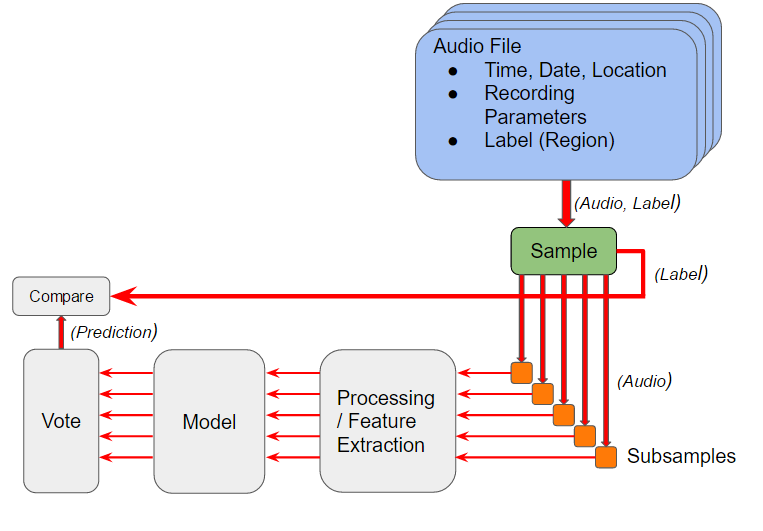
\includegraphics[width=0.9\linewidth]{pred_flow}
\end{figure}
\subsection{Locations}
The system is trained to recognize the following 7 locations:
\begin{enumerate}[label=\arabic*.]
\addtocounter{enumi}{-1}
\item Arrillaga Gym
\item Bytes Caf\'e
\item Circle of Death
    \subitem Intersection of Escondido and Lasuen
\item Huang Lawn
\item The Oval
\item Rains Graduate Housing
\item Tressider Memorial Union
\end{enumerate}
These locations represent the route a typical graduate engineering student living at Rains might take on a typical day. Locations 0,1, and 6 are indoors whereas Locations 2,3,4, and 5 are outdoors.


\section{Data Collection}\label{Data}
\subsection{Audio Format}\label{AudioFormat}
Data is collected using the \texttt{HI-Q MP3 REC (FREE)} application as noted in Section \ref{HwSw}. This application is freely available on the Google Play Store. Monophonic Audio is recorded without preprocessing and postprocessing at a sample rate of 44.1 kHz.
\subsection{Data Collection}
Initial training data was over a period of 2 days. Data was gathered at each location an equal number of times. Each data collection event followed the following procedure:
\begin{enumerate}
\item Configure \texttt{HI-Q MP3 REC (FREE)} to record audio as in \ref{AudioFormat}.
\item Hold the Android recording device away from body with no obstructions of the microphone
\item Stand in a single location throughout the recording
\item Record for 1 minute
\item Throw away recording if person recording interferes with the environment in some way (talks to a bystander, causes a bicycle crash, heckles passerby, etc...) 
\item Split recording into 10-second-long samples
\end{enumerate}
In total, we gathered 61 samples per location for a total of 432 samples. Roughly half of these samples were collected after 6pm; the other half were collected between 11am and 4pm.

\section{Audio Features}
We have investigated the use of the following features:
\begin{itemize}
\item Mean Amplitude in Time Domain
\item Variance of Amplitude in Time Domain
\item Fourier Transform
\item Autocorrelation (ACF)
\item SPED
\item Mel-frequency cepstral coefficients (MFCCs)
\end{itemize}
We binned the Fourier Transform into 40 bins for use as features. We used the first 40 lags in the Autocorrelation of each signal to use as features. The MFCC and SPED features are described in the following subsection.

\subsection{MFCC}
MFCCs are commonly used to characterize structured audio such as speech and music in the frequency domain, often as an alternative to the Fourier Transform \cite{Chu},\cite{Chu2Env},\cite{guo2003content},\cite{aucouturier2007bag}. Calculating the MFCCs proceeds in the following manner\cite{rabiner1993fundamentals}:
\begin{enumerate}
\item Divide the signal into short windows in the time domain
\item For each windowed signal:
    \begin{enumerate}
    \item Take the Fast Fourier Transform (FFT)
    \item Map powers of the FFT onto the mel scale
    \item Take the logarithm of the resultant mapping
    \item Take the discrete cosine transform (DCT) of the log mapping at a certain number of frequencies
    \item Output the resulting DCT
    \end{enumerate}
\end{enumerate} 
The calculation of MFCCs is available in the \texttt{scikits.talkbox} Python package. We chose to calculate 13 MFCCs over 5 ms windows for each input. This creates 13 MFCCs for each window of the input. We then take the mean over all windows to create 13 MFCC features for a given input.
\subsection{SPED}
SPED, Subband Peak Energy Detection, is a method of finding consistent sources of energy (in frequency) over time. First, a spectrogram is generated using time-windowed FFTs on the time-domain signal. The result is the energy of the signal as a function of both time and frequency. SPED then finds the peaks across frequency as defined by some window size. 

A local maximum is marked '1', and all other elements are zero. Finally, this matrix is summed across time to give a rough histogram of local maxima as a function of frequency. Finally, because of the fine resolution of the FFT in frequency, we use bin the results according to a log scale.

The idea behind this method is to find low-SNR energy sources that produce a coherent signal. For example, a motor or fan may produce a quiet but consistent sum of tones. In an FFT, this may or may not be visible. However, it will likely result in local maxima over time. Since all maxima are weighted equally, SPED seeks to expose all consistent frequencies regardless of their power. Below, we show a SPED output for Bytes Caf\'e and Arrillaga Gym across different days and different areas. 
\begin{figure}[H]
	\centering
	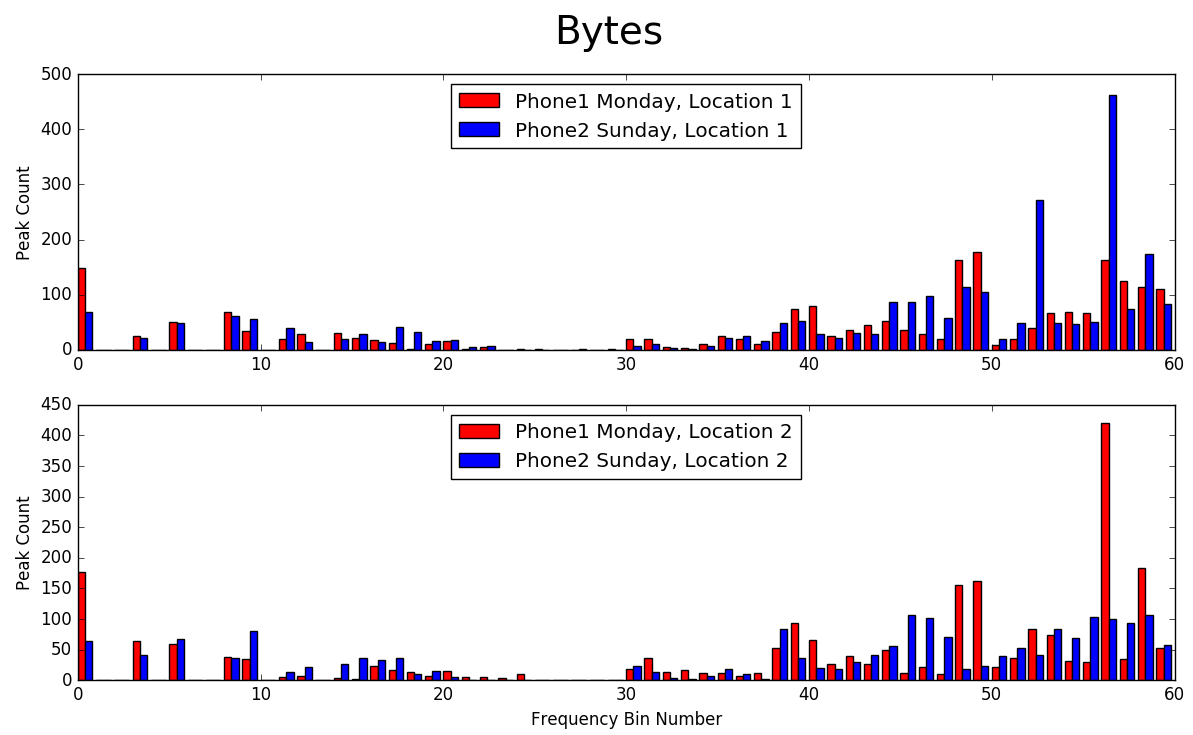
\includegraphics[width=0.9\linewidth]{bytes_sped}
\end{figure}
\begin{figure}[H]
	\centering
	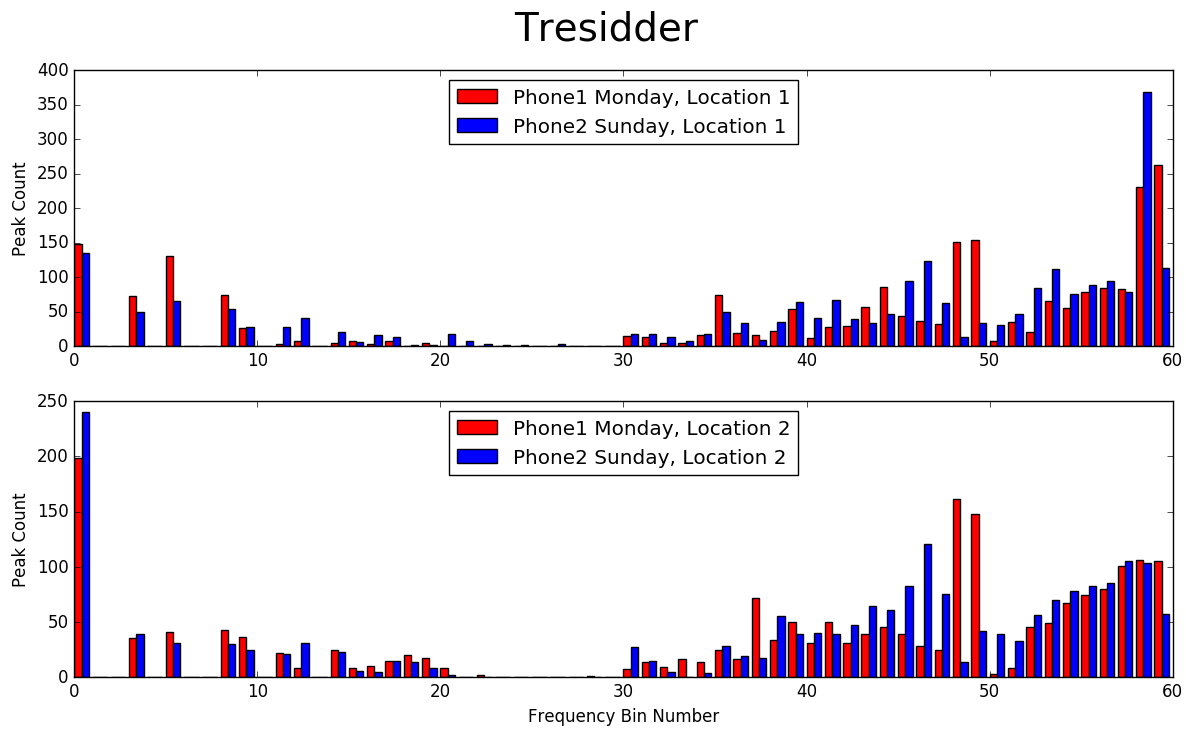
\includegraphics[width=0.9\linewidth]{tressider_sped}
\end{figure}

\section{Preliminary Methods and Results}
We investigate Logistic Regression, SVM with a linear kernel, and SVM with a radial basis kernel function, experimenting with different subsets of features with each algorithm. In reference to the system flow in Section \ref{Signal Flow}, we choose 10-second samples and 2-second subsamples. So, a sample will be input to the system, 5 predictions (1 for each subsample) will be made, and finally the most frequent prediction will be output.  For training, we randomly shuffle the samples and use $2/3$ as training and $1/3$ as testing. To make valid comparisons across different training instances, we reset to a given random number generator seed whenever shuffling the samples. The training flow diagram is similar to the prediction flow diagram:
\begin{figure}[H]
\centering
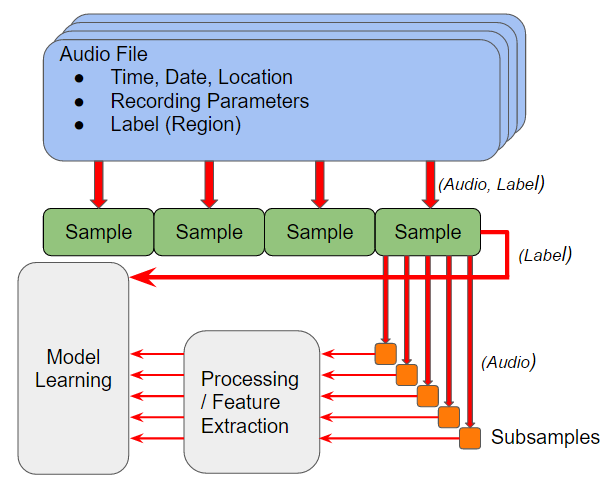
\includegraphics[width=0.9\linewidth]{train_flow}
\end{figure}

We train each classifier on subsamples. So, for each training sample, we generate 5 training subsamples. However, we calculate training and testing error based on entire samples, using the aforementioned procedure. Some of the results are below with different error penalty terms $C$:
\begin{figure}[H]
\centering
\begin{subfigure}{0.5\linewidth}
\centering
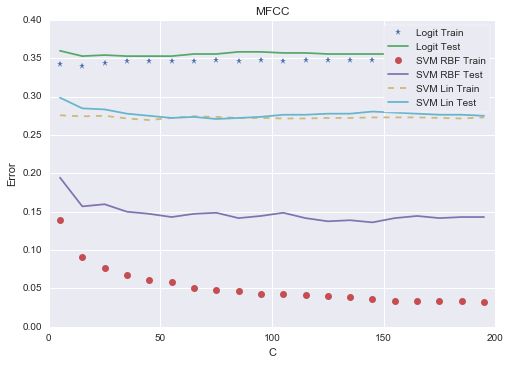
\includegraphics[width=0.9\linewidth]{MFCC_Err}
\end{subfigure}\hfill
\begin{subfigure}{0.5\linewidth}
\centering
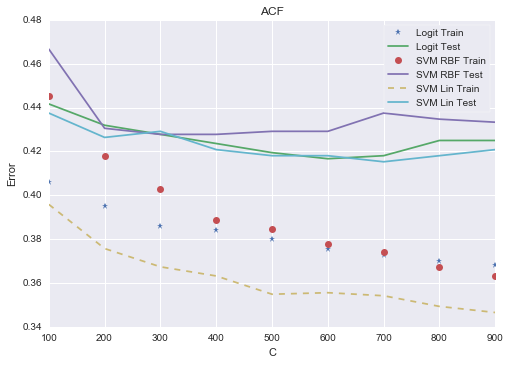
\includegraphics[width=0.9\linewidth]{ACF_Err}
\end{subfigure}
\end{figure}

\begin{figure}[H]
\centering
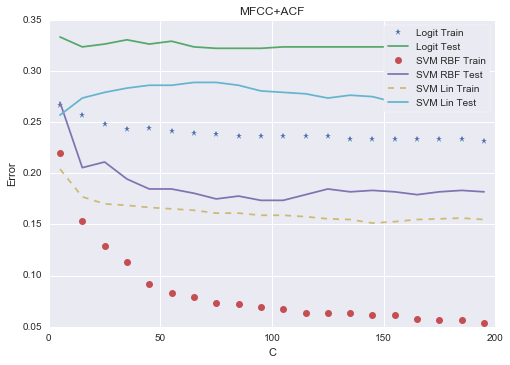
\includegraphics[width=0.45\linewidth]{MFCC_ACF_Err}
\end{figure}
From these results, we conclude that the most promising simple classification algorithm is using MFCC features to train an RBF-kernel SVM with a penalty parameter $C=15$, despite the considerable gap between training and testing errors. Surprisingly, adding features in conjunction with MFCC features does not seem to improve performance for any of the simple classifiers we tried.

Note we also tested other features as well that due to poor performance have not been plotted here. We saw that the FFT features did not improve upon performance when combined with the ACF features. In retrospect, this somewhat makes sense because the ACF can be calculated directly from the FFT. Somewhat surprisingly, we saw extremely bad performance when using just FFT features. For some reason, all learning algorithms would classify all inputs as Bytes Caf\'e. This may merit further investigation later.

Also, we saw that the SPED features we calculated worked reasonably well when used in conjunction with a Linear SVM, obtaining about $20\%$ test error. However, it performed quite poorly using the RBF-kernel SVM that worked well with the MFCC features. In order to incorporate both, we will explore the possibility of 'Mixture of Experts' to intelligently combine the two. Furthermore, calculation of the SPED features is still rather inefficient. By exercising feature analysis, we may be able to determine certain frequency ranges that are most useful in order to reduce computations and well as feature size. 

\section{Future Work}
We plan on gathering more data points at different days of the week in order to evaluate better the generalization of our system. We also plan to investigate ensemble methods in order to combine features with MFCC in a way that improves performance rather than degrades it. If we cannot force our current feature selection to work well together, we may evaluate some of the other features that have been mentioned in the Literature, including time domain features.
% references section

% can use a bibliography generated by BibTeX as a .bbl file
% BibTeX documentation can be easily obtained at:
% http://mirror.ctan.org/biblio/bibtex/contrib/doc/
% The IEEEtran BibTeX style support page is at:
% http://www.michaelshell.org/tex/ieeetran/bibtex/
%\bibliographystyle{IEEEtran}
% argument is your BibTeX string definitions and bibliography database(s)
%\bibliography{IEEEabrv,../bib/paper}
%
% <OR> manually copy in the resultant .bbl file
% set second argument of \begin to the number of references
% (used to reserve space for the reference number labels box)
\bibliographystyle{IEEEtran}
\bibliography{CS229_Progress_report}
\raggedbottom



\end{document}
